\documentclass[11pt,a4paper]{article}

\usepackage[utf8]{inputenc}
\usepackage[spanish]{babel}

\usepackage{enumitem}

\usepackage{cite}

\usepackage{url}
\usepackage[hidelinks]{hyperref}

\usepackage{graphicx}
\usepackage{color}

\usepackage{caption}

\bibliographystyle{plain}

\title{Análisis del \emph{malware CTB-Locker}}

\author{\begin{tabular}[center]{c}
          Ignacio Ballesteros González \\
          \small w140062 \\
          \small 05448027V \\
        \end{tabular}
      }
\date{\today}

\begin{document}

\maketitle
\tableofcontents
\normalsize
\begin{abstract}
  Primera práctica de la asignatura de \emph{Seguridad de las
    Tecnologías de la Información}. Se realizará el estudio de una
  muestra del código malicioso \emph{CTB-Locker}. Se ha elegido la
  opción \textit{(a)} de estudio en base a las normas establecidas.

  \begin{center}
    $((5448027 * 485750 )~mod~331) = 73$
  \end{center}
\end{abstract}

\section{Introducción}
\label{sec:intro}
\emph{CTB-Locker} es un malware que cifra los ficheros de la víctima y pide una compesación
económica para recuperer los archivos cifrados.\cite{FSecure}

\begin{description}[leftmargin=9em,style=nextline]
  \item[Código malicioso] \emph{CTB-Locker}
  \item[Tipo] Toyano
  \item[Familia] Secuestrador/Rescatador \emph{(ramsonware)}
\end{description}

\section{Ficha resumen}

\begin{description}[leftmargin=5.5em,align=right,labelwidth=2cm]
\item[Denominación] \emph{CTB-Locker}
\item[Origen/autor] Tapkin. \cite{Point}
\item[Destinatario] Usuarios comunes. Empresas. Países de habla inglesa. \cite{Sophos}
\item[Fecha de lazamiento] Publicado en foros rusos el 10 de junio de 2014 \cite{Point}
\item[Fecha de descubrimiento] 4 de febrero de 2015 \cite{Point}
\item[Tipo de código malicioso] \emph{Ramsonware}
\end{description}

  \begin{center}
    \textbf{Funcionamiento general}
  \end{center}

\begin{description}[leftmargin=5.5em,align=right,labelwidth=2cm]  
\item[Modo de infección] Campañas de Spam en fichero infectados. \cite{Point}
\item[Modo de replicación] No aplica.
\item[Modo de propagación] Campañas de \emph{phising}.
\item[Modo de ocultación] No aplica.
\item[Ejecución de la carga] Ficheros infectados.
\end{description}
  
  \begin{center}
    \textbf{Tiempo de vulnerabilidad relacionada}
  \end{center}

  Las infecciones se han producido en periodo que abarca desde finales de enero de 2015 a mediados de febrero de 2015. \cite{FS2}

    \begin{center}
    \textbf{Modo de desinfección}
  \end{center}

La compañía F-Secure ha incluido el mecanismo de desinfección en su herramienta general.

  \begin{center}
    \textbf{Ejemplo de ataque donde se ha empleado}
  \end{center}

Ver Figura \ref{fig:1} y \ref{fig:2}
  
\begin{figure}
  \caption{Ejemplo de correo de Spam con infección}
  \label{fig:1}
  \centering
  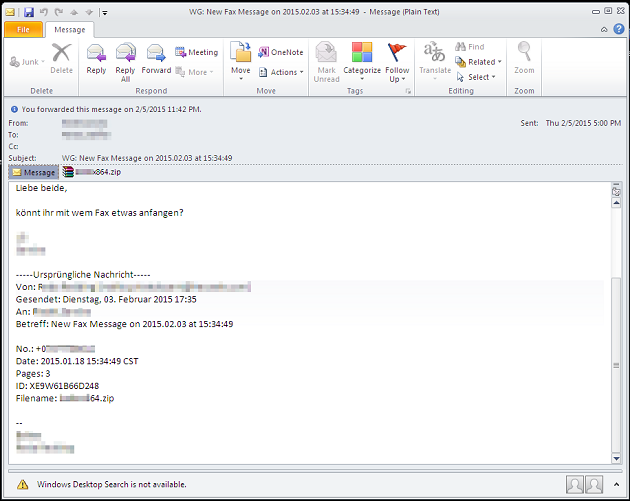
\includegraphics[width=1\textwidth]{spam2.PNG}
\end{figure}


\begin{figure}
  \caption{Pantalla una vez están los archivos cifrados.}
  \label{fig:2}
  \centering
  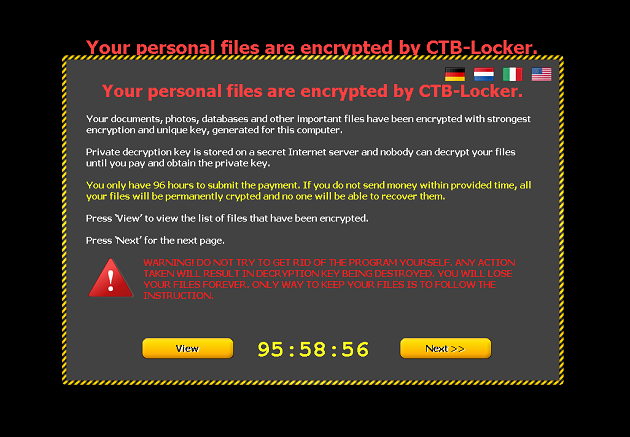
\includegraphics[width=\textwidth]{ctblocker_lockscreen.png}
\end{figure}

  \begin{center}
    \textbf{Medidas de seguridad tomadas tras su descubrimiento}
  \end{center}

\begin{enumerate}
\item Uso de herramientas de detección del \emph{malware}.
\item Educación en la prevención de campañas de \emph{phising}.
\end{enumerate}

  \begin{center}
    \textbf{Resto de miembros de su familia}
  \end{center}

Asociado a \emph{CTB-Locker} Kaspersky designa a la familia de \emph{malware} como \emph{Trojan-Ransom.Win32.Onion}.

A veces se le conoce también como \emph{Dalexis} \cite{FS2}

Relacionado con la familia \emph{Cryptolocker} \cite{FSecure}

Por otro lado, se han creado imitaciones del \emph{malware} como \emph{Poliglot} \cite[p.~11]{Kas16}

  \begin{center}
    \textbf{Otra información relevante}
  \end{center}

\emph{CTB-Locker} comprimía los archivos con una herramienta propia antes de cifrarlos. \cite{Point}

\section{Conclusiones}
\label{sec:conclusiones}

El \emph{malware} \emph{CTB-Locker} tuvo una fugaz aparición enmarcada en la ola de ramsonware de 2015. Cotenía mecanismos novedosos para el cifrado de los ficheros y a su vez la calidad de desarrollo era elevada.

\bibliography{malware}

\end{document}
